\documentclass[11pt]{scrartcl}
\usepackage[utf8]{inputenc}
\usepackage[sexy]{evanchen} 
\usepackage{graphicx}
\graphicspath{{8 Outsource K Math/Gambar/}}

\title{Lingkaran}
\author{Azzam and Akeyla}
\date{Februari 2024}

\begin{document}

\maketitle

\section{Definisi dan Istilah}
Lingkaran adalah kumpulan titik yang berjarak sama ke sebuah titik.
\begin{figure}[h]
    \centering
    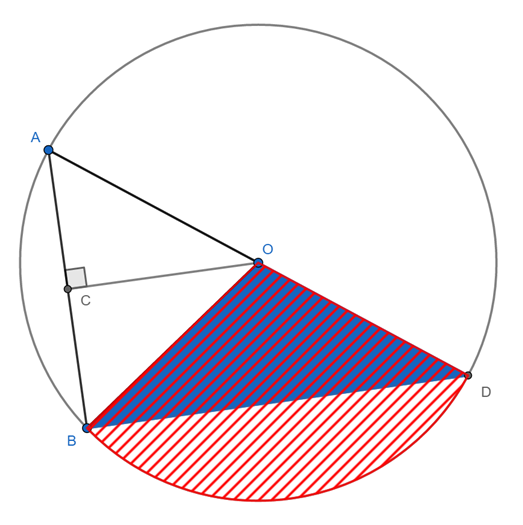
\includegraphics[width=0.5\linewidth]{lingkaran.png}
\end{figure}

Istilah pada lingkaran:
\begin{enumerate}
    \item 	Titik pusat (Titik $O$)
	\item Jari-jari ($OA, OB, OD$)
	\item Diameter ($AD$)
	\item Juring (Semua yang diarsir merah)
	\item Tembereng (Yang diarsir merah tetapi tidak diarsir biru)
	\item Apotema ($OC$)
	\item Tali busur ($AB, BD$ yang lurus)
	\item Busur ($AB, BD$ yang melengkung)
\end{enumerate}

Luas dan keliling lingkaran
\begin{enumerate}
    \item Luas = $\pi r^2$ dengan $r$ adalah panjang jari-jari
    \item Keliling = $\pi d=2\pi r$ dengan $d$ adalah panjang diameter 
\end{enumerate}

\subsection{Latihan Soal}
\begin{problem}
    Diberikan persegi dengan panjang sisi $10$ dan dua buah seperempat lingkaran. Berapakah luas daerah yang diarsir (yang warnanya lebih gelap)?
    \begin{figure}[h]
        \centering
        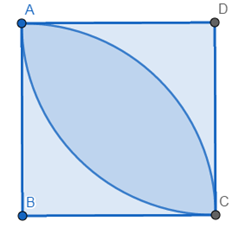
\includegraphics[width=0.3\linewidth]{luaspersekutuanduaseperempatlingkaran.png}
    \end{figure}
\end{problem}

\begin{problem}
(Chile MO 1989) Diberikan sebuah segitiga siku-siku dengan panjang sisi $a, b,$ dan $c$ dengan $c$ adalah panjang sisi miringnya. Tiga setengah lingkaran digambar dengan diameter yang merupakan ketiga sisi segitiga tersebut seperti yang ditunjukkan pada gambar. Diketahui bahwa luas daerah berwarna ungu adalah $X$ dan $Y$. Nyatakanlah nilai $X + Y$ dalam $a, b,$ dan $c$.
\begin{figure}[h]
    \centering
    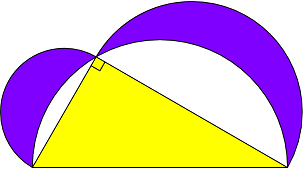
\includegraphics[width=0.5\linewidth]{ChileMO1989P3.png}
\end{figure}
\end{problem}

\begin{problem}
(AMC 12A 2003) Sebuah setengah lingkaran dengan diameter $1$ berada di atas sebuah setengah lingkaran berdiameter $2$ seperti pada gambar di bawah. Daerah yang diarsir di dalam setengah lingkaran kecil tetapi di luar setengah lingkaran besar disebut sebagai sabit. Luas daerah sabit adalah ...
    \begin{figure}[h]
        \centering
        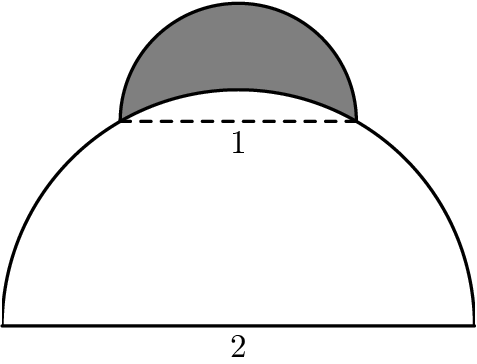
\includegraphics[width=0.5\linewidth]{AMC12200315.png}
    \end{figure}
\end{problem}

\section{Properti Lingkaran}
\begin{enumerate}
    \item Panjang diameter adalah dua kali panjang jari-jari
    \item Besar sudut keliling adalah setengah dari sudut pusat yang menghadap busur yang sama
    \item Jika $AB$ adalah diameter lingkaran dan $C$ adalah titik di keliling lingkaran, maka $\angle{ACB}$ siku-siku.
    \item Dua sudut keliling yang menghadap busur yang sama memiliki besar sudut yang sama
    \item Dua (tali) busur panjangnya sama -> Sudut keliling/pusat yang menghadap kedua busur tersebut besarnya sama
    \item Misalkan garis $l$ menyinggung lingkaran yang berpusat di $O$ pada titik $A$ maka $OA$ akan tegak lurus garis $l$.
	\item Titik $A$ terletak di luar lingkaran yang berpusat di $O$. Tarik dua garis singgung lingkaran dari titik $A$ yang menyinggung di titik $P$ dan $Q$. Maka, $AP = AQ$ dan $\angle{APO}= \angle{BPO}$
	\item Misal $l$ adalah garis yang menyinggung lingkaran di $P$. Titik $A$ dan $B$ terletak di lingkaran dan titik $X$ terletak di garis $l$ sedemikian hingga $\angle{XPA}< \angle{XPB}$.  Maka, $\angle{XPA}= \angle{PBA}$.
	\item Jika $A, B, C, D$ adalah empat titik pada lingkaran dengan urutan tersebut, maka $\angle{ABC}+ \angle{ADC}=180^{\circ}$.
    \item Jika $AB$ dan $CD$ adalah dua tali busur yang berpotongan di $X$, maka $AX\cdot XB=CX\cdot XD$. Hal kebalikannya juga berlaku.
\end{enumerate}

\subsection{Latihan Soal}
\begin{problem}
    Dua buah garis singgung ditarik dari titik $A$ ke sebuah lingkaran. Kedua titik singgung, $B$ dan $C$ membagi lingkaran menjadi dua busur dengan rasio panjang $2:3$. Besar sudut $\angle{BAC}$ adalah ...
\end{problem}

\begin{problem}
    Gambar di bawah menunjukkan sebuah lingkaran yang berpusat di $O$. Diketahui bahwa $\angle{ABE}+\angle{ACE}+\angle{ADE}=102^{\circ}$. Besar sudut $\angle{AOE}$ adalah ...
    \begin{figure}[h]
        \centering
        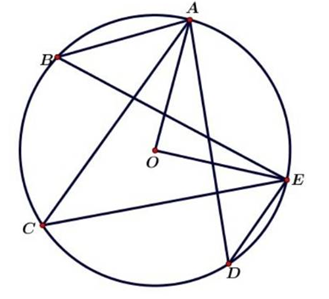
\includegraphics[width=0.5\linewidth]{anglechasinglingkaran1.png}
    \end{figure}
\end{problem}

\begin{problem}
    Diberikan segitiga $ABC$ siku-siku di $B$ dengan $AB = 20, BC = 21$, dan $AC = 29$. Jika $M$ adalah titik tengah $AC$, tentukan panjang $BM$.
\end{problem}

\begin{problem}
    Garis $AD$ adalah diameter setengah lingkaran yang berpusat di $O$. Titik $B$ dan titik $C$ keduanya terletak pada setengah lingkaran sehingga garis $AC$ tegak lurus $BO$. Jika diketahui $\angle{CAD} = 50^{\circ}$, hitunglah sudut yang dibentuk antara garis $AC$ dan $BD$.
\end{problem}

\begin{problem}
   Perhatikan gambar di bawah.
    \begin{figure}[h]
        \centering
        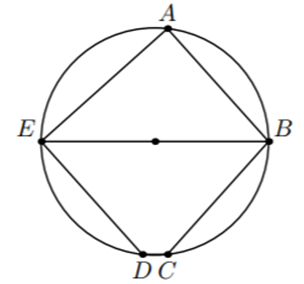
\includegraphics[width=0.3\linewidth]{anglechasinglingkaranlimatitik.png}
    \end{figure}
    Diameter $EB$ sejajar dengan $DC$. $AB$ sejajar dengan $DE$. Besar sudut $\angle{AEB}$ dan $\angle{ABE}$ membentuk rasio $4:5$. Besar dari sudut $\angle{BCD}$ adalah ...
\end{problem}

\subsection{Latihan Soal Lingkaran yang Menyinggung}

\begin{problem}
    (AIME II 2014) Lingkaran $C$ dengan jari-jari $2$ memiliki diameter $AB$. Lingkaran $D$ menyinggung lingkaran $C$ secara internal pada titik $A$. Lingkaran $E$ menyinggung lingkaran $C$ secara internal, menyinggung lingkaran $D$ secara eksternal, dan menyinggung $AB$. Jari-jari lingkaran $D$ tiga kali panjang jari-jari lingkaran $E$ dan dapat dituliskan dalam bentuk $\sqrt{m} - n$ dengan $m$ dan $n$ keduanya adalah bilangan asli. Tentukan nilai $m + n$.
\end{problem}

\begin{problem}
%4\pi\sqrt{3}
%https://artofproblemsolving.com/community/c5h1781124p11736322
    Gambar di bawah menunjukkan tigabelas lingkaran berjari-jari $1$ yang saling menyinggung satu sama lain dan juga menyinggung sebuah lingkaran besar secara internal. Luas dari daerah yang ada di dalam lingkaran besar tetapi di luar ketigabelas lingkaran kecil (yakni, luas daerah yang diarsir) adalah ...
    \begin{figure}[h]
        \centering
        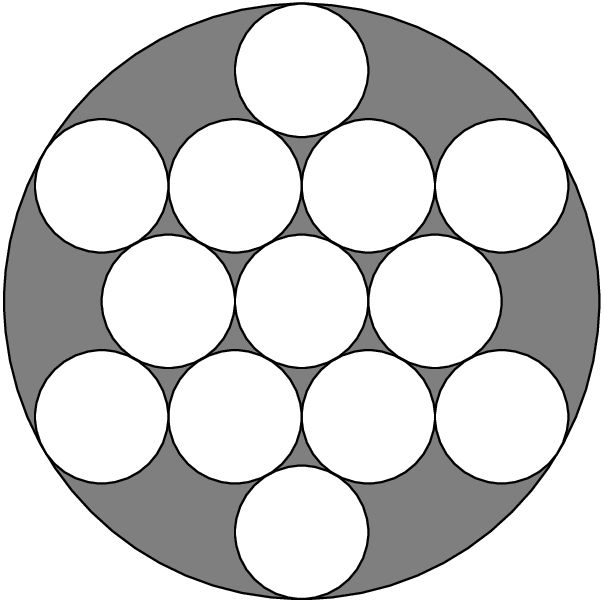
\includegraphics[width=0.3\linewidth]{luas13lingkaran.png}
    \end{figure}
\end{problem}

\begin{problem}
Lingkaran $A$ dan $B$ yang keduanya memiliki panjang jari-jari $1$ bersinggungan secara eksternal. Empat lingkaran $P, Q, R, S$ yang memiliki panjang jari-jari $r$ diposisikan sedemikian hingga $P$ menyinggung $A, B, Q,$ dan $S$ secara eksternal, $Q$ menyinggung $P, B,$ dan $R$ secara eksternal, $R$ menyinggung $A, B, Q,$ dan $S$ secara eksternal, dan $S$ menyinggung $P, A,$ dan $R$ secara eksternal. Tentukan panjang $r$.
\begin{figure}[h]
    \centering
    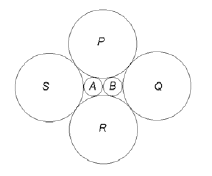
\includegraphics[width=0.5\linewidth]{BelandaMO2004P2.png}
\end{figure}
\end{problem}

\begin{problem}
    (AMC 2017 12A) Pada gambar di bawah, diberikan dua buah setengah lingkaran yang berpusat di $A$ dan $B$ yang secara berturut-turut memiliki panjang jari-jari $2$ dan $1$. Kedua setengah lingkaran ini dibangun di dalam sebuah setengah lingkaran yang berdiameter $JK$ dan diameter dari kedua lingkaran kecil ini berhimpit dengan diameter setengah lingkaran besar. Kedua setengah lingkaran kecil ini bersinggungan secara eksternal satu sama lain dan menyinggung setengah lingkaran besar secara internal. Sebuah lingkaran yang berpusat di titik $P$ menyinggung dua setengah lingkaran kecil secara eksternal dan menyinggung setengah lingkaran besar secara internal. Panjang jari-jari lingkaran yang berpusat di titik $P$ tersebut adalah ...
    \begin{figure}[h]
        \centering
        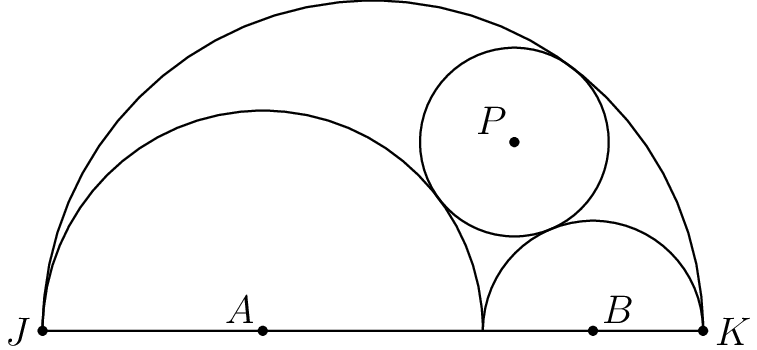
\includegraphics[width=0.5\linewidth]{2017AMC12AP16.png}
    \end{figure}
\end{problem}

\section{Segiempat Siklik}
Sebuah segiempat dikatakan sebagai segiempat siklik apabila keempat titik sudutnya terletak di keliling sebuah lingkaran. 
\begin{figure}[h]
    \centering
    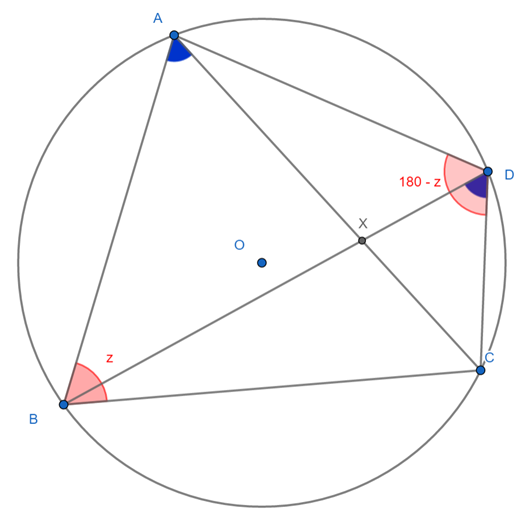
\includegraphics[width=0.5\linewidth]{siklik.png}
\end{figure}
Segiempat siklik memiliki beberapa properti berikut:
\begin{enumerate}
    \item Dua sudut keliling yang menghadap busur yang sama memiliki besar yang sama.
	\item Dua sudut keliling yang berseberangan jumlahnya adalah $180^{\circ}$.
	\item (Power of Point) $AX\cdot XC=BX \cdot XD$.
	\item (Dalil Ptolemy) $AC \cdot BD=AD \cdot BC + AB\cdot CD$.
    \item (Brahmagupta) Luas dari $ABCD$ adalah $\sqrt{(s-a)(s-b)(s-c)(s-d)}$ dengan $s=\dfrac{a+b+c+d}{2}$.
\end{enumerate}

\subsection{Latihan Soal}
\begin{problem}
    % Ptolemy, 10
    Misalkan $P$ adalah titik yang terletak di busur minor $BC$ dari lingkaran luar sebuah segitiga sama sisi $ABC$. Jika $PB=3$ dan $PC=7$, panjang $PA$ adalah ...
\end{problem}

\begin{problem}
    Titik $A$ dan $C$ terletak di keliling sebuah lingkaran yang berpusat di $O$. Titik $B$ terletak sedemikian rupa sehingga $BA$ dan $BC$ adalah garis singgung lingkaran dan $ABC$ adalah segitiga sama sisi. Jika $BO$ memotong lingkaran di $D$, perbandingan panjang $BD:BO$ adalah …
\end{problem}

\begin{problem}
    (Chile MO 2015) Diberikan sebuah segiempat $ABCD$ yang siklik. Diketahui bahwa $DA = BC = 2$ dan $AB = 4$. Titik $E$ adalah perpotongan $BC$ dan $DA$. Diketahui bahwa $\angle AEB = 60^{\circ}$ dan $CD < AB$. Hitunglah jari-jari dari lingkaran tersebut.
\end{problem}

\begin{problem}
    (AIME II 2011) Sebuah lingkaran yang berpusat di $O$ memiliki jari-jari sepanjang $25$. Tali busur $AB$ memiliki panjang $30$ dan tali busur $CD$ dengan panjang $14$ berpotongan di titik $P$. Jarak antara titik tengah kedua tali busur tersebut adalah $12$. Diketahui bahwa nilai $OP^2$ dapat dinyatakan dalam bentuk $\frac{m}{n}$ dengan $m$ dan $n$ keduanya merupakan bilangan asli yang relatif prima. tentukan sisa bagi saat $m + n$ dibagi oleh $1000$.
\end{problem}

\begin{problem}
    (AMC 2016 10A) Sebuah segiempat memiliki empat titik sudut yang terletak di sebuah lingkaran. Apabila panjang tiga dari empat sisi segiempat ini memiliki panjang $200$ dan panjang jari-jari lingkaran adalah $200\sqrt{2}$, maka panjang dari sisi keempat dari segiempat ini adalah ...
\end{problem}

\begin{problem}
    Pada segitiga $ABC$, $AB=13$, $BC=14$, dan $CA=15$. Tiga titik berbeda $D$, $E$, dan $F$ berada di segmen garis $BC$, $CA$, dan $DE$ sedemikian hingga $AD$ tegak lurus $BC$, $DE$ tegak lurus $AC$, dan $AF$ tegak lurus $BF$. Panjang dari $DF$ adalah ...
\end{problem}

\end{document}